\documentclass[9pt]{article}
\usepackage[a4paper,landscape,margin=10mm]{geometry}
\usepackage{fontspec}
\setmainfont{DejaVu Sans}
\usepackage{tikz}
\usetikzlibrary{arrows.meta,positioning,calc,backgrounds}
\usepackage{xcolor}
\pagestyle{empty}
\definecolor{navy}{HTML}{182D4D}
\definecolor{teal}{HTML}{007F86}
\definecolor{ink}{HTML}{2B3545}
\definecolor{softblue}{HTML}{EEF4FA}
\definecolor{softmint}{HTML}{E8F6F2}
\definecolor{softgold}{HTML}{FFF6E3}
\definecolor{softgray}{HTML}{F4F6F8}
\definecolor{redbrown}{HTML}{A35136}
\begin{document}
\noindent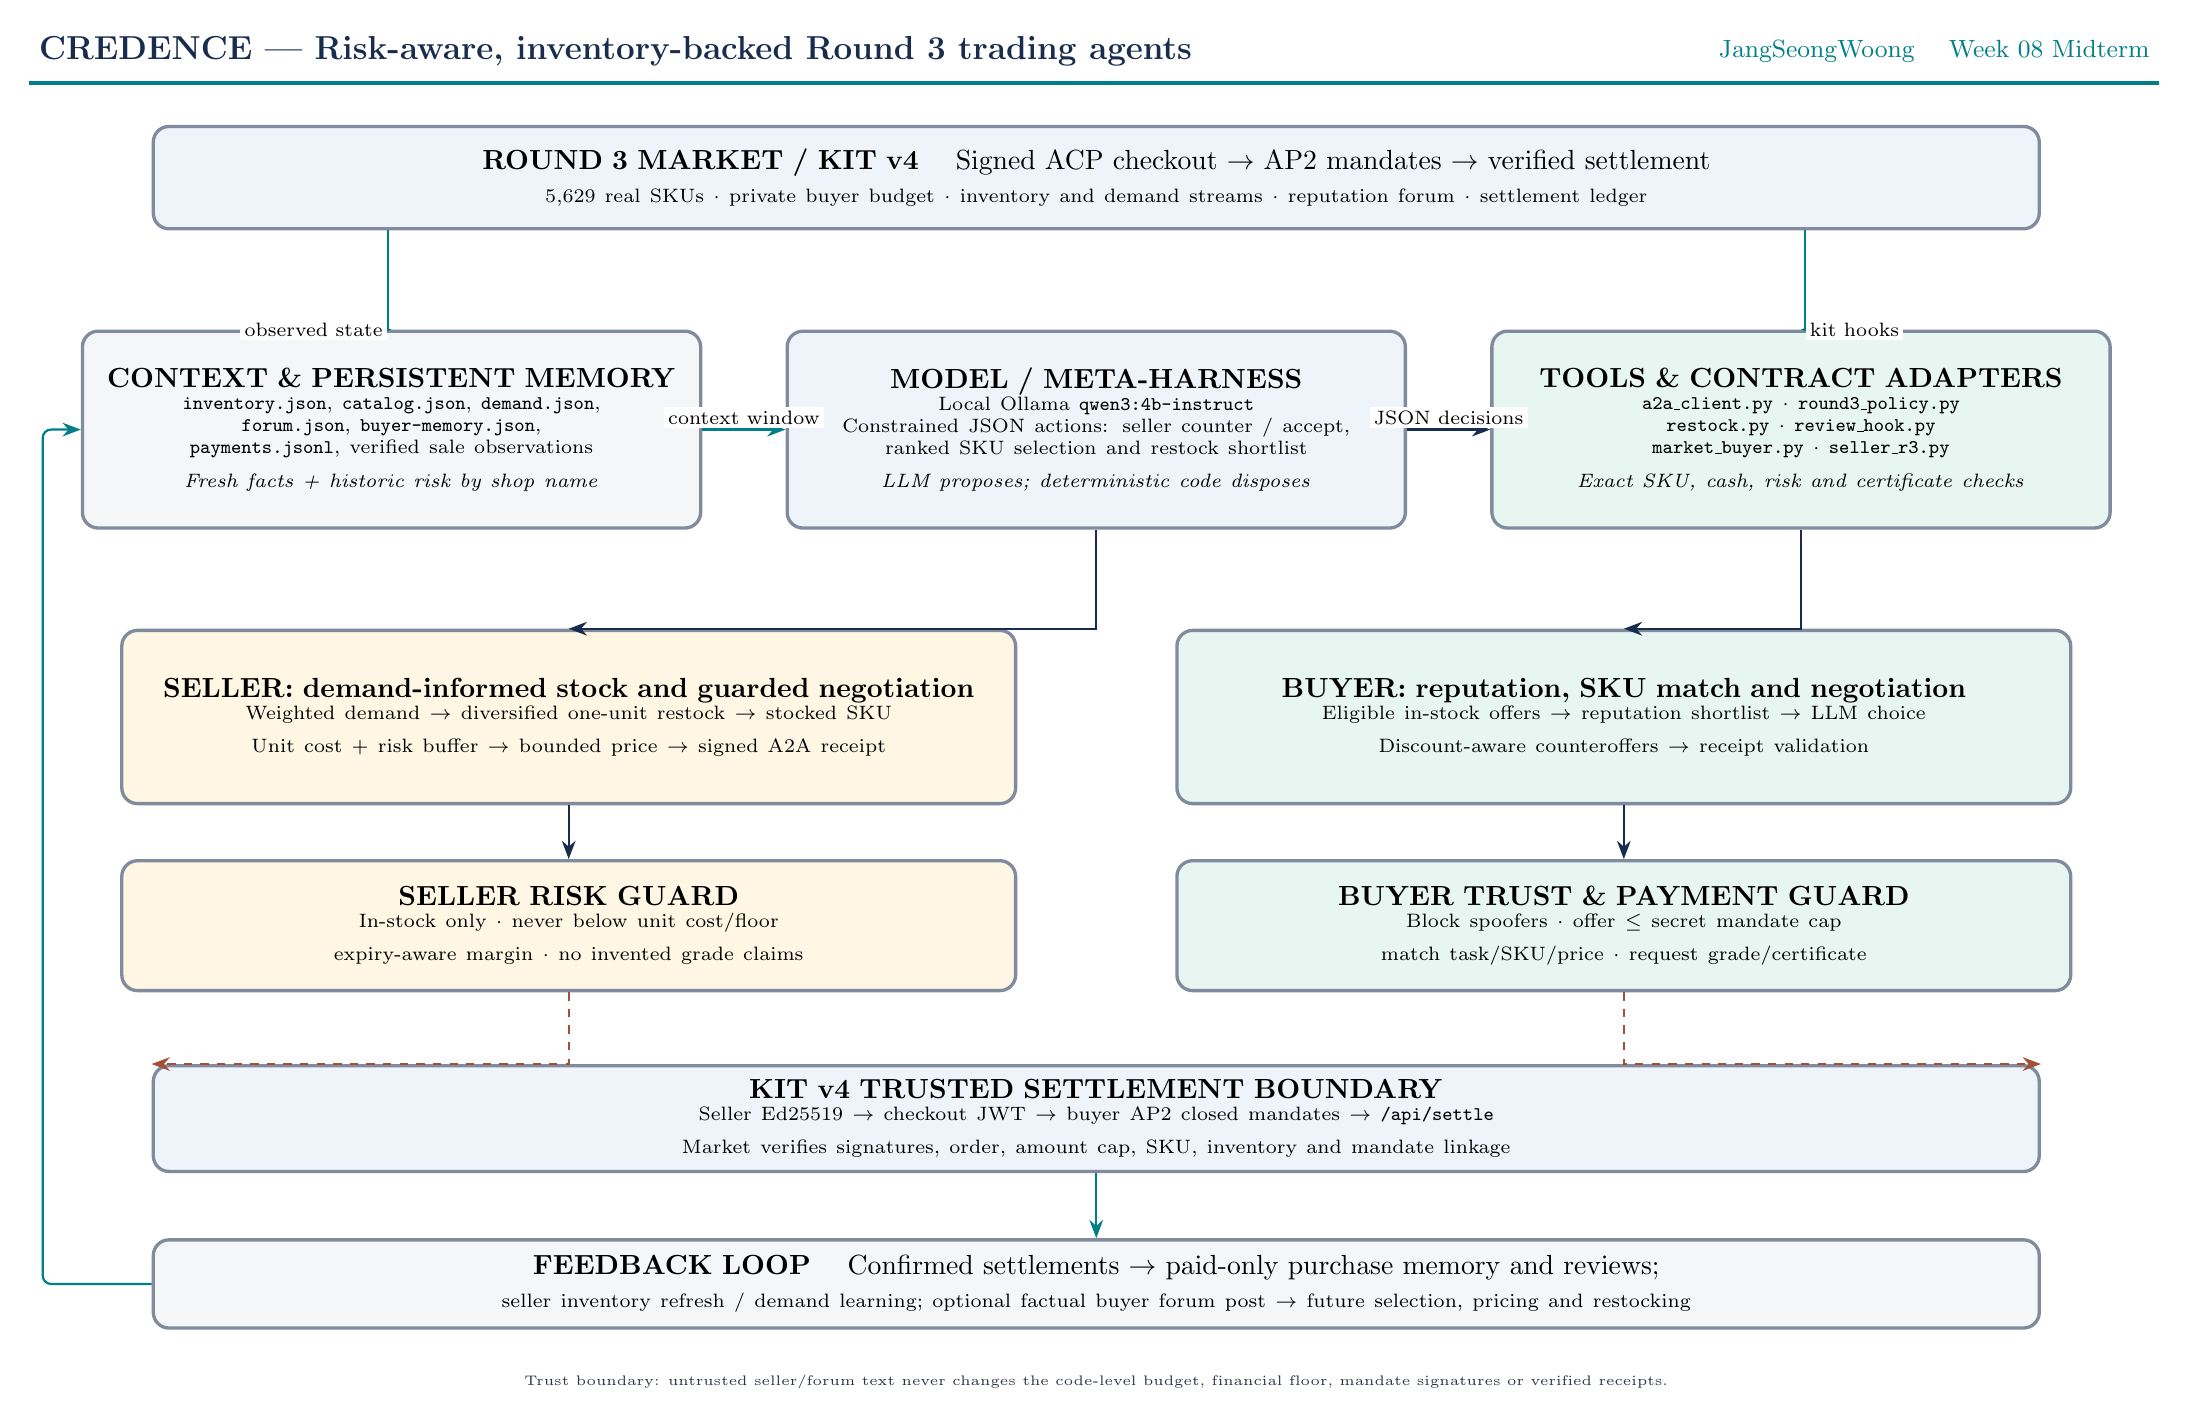
\begin{tikzpicture}[x=1cm,y=1cm,
  box/.style={draw=navy!55,rounded corners=2mm,very thick,fill=white,align=center,inner sep=5pt},
  data/.style={-Stealth,thick,draw=teal},
  control/.style={-Stealth,thick,draw=navy},
  verify/.style={-Stealth,thick,draw=redbrown,dashed},
  label/.style={font=\scriptsize,fill=white,inner sep=1.5pt,align=center},
  title/.style={font=\bfseries\large,text=navy},
  sub/.style={font=\scriptsize,text=ink,align=center},
  tiny/.style={font=\tiny,text=ink,align=center}
]
\node[title,anchor=west] at (.25,17.45) {CREDENCE | Risk-aware, inventory-backed Round 3 trading agents};
\node[font=\small,text=teal,anchor=east] at (27.3,17.45) {JangSeongWoong \quad Week 08 Midterm};
\draw[teal,line width=1.2pt] (.25,17.05)--(27.3,17.05);
\node[box,fill=softblue,text width=23.6cm,minimum height=1.3cm] (market) at (13.8,15.85)
 {\textbf{ROUND 3 MARKET / KIT v4} \quad Signed ACP checkout \(\to\) AP2 mandates \(\to\) verified settlement\\
  \scriptsize 5,629 real SKUs \(\cdot\) private buyer budget \(\cdot\) inventory and demand streams \(\cdot\) reputation forum \(\cdot\) settlement ledger};
\node[box,fill=softgray,text width=7.5cm,minimum height=2.5cm] (context) at (4.85,12.65)
 {\textbf{CONTEXT \& PERSISTENT MEMORY}\\
 \scriptsize \texttt{inventory.json}, \texttt{catalog.json}, \texttt{demand.json},\\
 \texttt{forum.json}, \texttt{buyer-memory.json},\\
 \texttt{payments.jsonl}, verified sale observations\\
 \scriptsize\textit{Fresh facts + historic risk by shop name}};
\node[box,fill=softblue,text width=7.5cm,minimum height=2.5cm] (model) at (13.8,12.65)
 {\textbf{MODEL / META-HARNESS}\\
 \scriptsize Local Ollama \texttt{qwen3:4b-instruct}\\
 \scriptsize Constrained JSON actions: seller counter / accept,\\
 ranked SKU selection and restock shortlist\\
 \scriptsize\textit{LLM proposes; deterministic code disposes}};
\node[box,fill=softmint,text width=7.5cm,minimum height=2.5cm] (tools) at (22.75,12.65)
 {\textbf{TOOLS \& CONTRACT ADAPTERS}\\
 \scriptsize \texttt{a2a\_client.py} \(\cdot\) \texttt{round3\_policy.py}\\
 \scriptsize \texttt{restock.py} \(\cdot\) \texttt{review\_hook.py}\\
 \scriptsize \texttt{market\_buyer.py} \(\cdot\) \texttt{seller\_r3.py}\\
 \scriptsize\textit{Exact SKU, cash, risk and certificate checks}};
\draw[data] (market.south west) ++(3,0) |- node[label,left]{observed state} (context.north);
\draw[data] (context.east) -- node[label,above]{context window} (model.west);
\draw[control] (model.east) -- node[label,above]{JSON decisions} (tools.west);
\draw[data] (market.south east) ++(-3,0) |- node[label,right]{kit hooks} (tools.north);
\node[box,fill=softgold,text width=11cm,minimum height=2.2cm] (seller) at (7.1,9.0)
 {\textbf{SELLER: demand-informed stock and guarded negotiation}\\
 \scriptsize Weighted demand \(\to\) diversified one-unit restock \(\to\) stocked SKU\\
 \scriptsize Unit cost + risk buffer \(\to\) bounded price \(\to\) signed A2A receipt};
\node[box,fill=softmint,text width=11cm,minimum height=2.2cm] (buyer) at (20.5,9.0)
 {\textbf{BUYER: reputation, SKU match and negotiation}\\
 \scriptsize Eligible in-stock offers \(\to\) reputation shortlist \(\to\) LLM choice\\
 \scriptsize Discount-aware counteroffers \(\to\) receipt validation};
\draw[control] (tools.south) |- (buyer.north);
\draw[control] (model.south) |- (seller.north);
\node[box,fill=softgold,text width=11cm,minimum height=1.65cm] (sellerGuard) at (7.1,6.35)
 {\textbf{SELLER RISK GUARD}\\
 \scriptsize In-stock only \(\cdot\) never below unit cost/floor\\
 \scriptsize expiry-aware margin \(\cdot\) no invented grade claims};
\node[box,fill=softmint,text width=11cm,minimum height=1.65cm] (buyerGuard) at (20.5,6.35)
 {\textbf{BUYER TRUST \& PAYMENT GUARD}\\
 \scriptsize Block spoofers \(\cdot\) offer \(\leq\) secret mandate cap\\
 \scriptsize match task/SKU/price \(\cdot\) request grade/certificate};
\draw[control] (seller.south) -- (sellerGuard.north);
\draw[control] (buyer.south) -- (buyerGuard.north);
\node[box,fill=softblue,text width=23.6cm,minimum height=1.3cm] (settle) at (13.8,3.9)
 {\textbf{KIT v4 TRUSTED SETTLEMENT BOUNDARY}\\
 \scriptsize Seller Ed25519 \(\to\) checkout JWT \(\to\) buyer AP2 closed mandates \(\to\) \texttt{/api/settle} \\
 \scriptsize Market verifies signatures, order, amount cap, SKU, inventory and mandate linkage};
\draw[verify] (sellerGuard.south) |- (settle.north west);
\draw[verify] (buyerGuard.south) |- (settle.north east);
\node[box,fill=softgray,text width=23.6cm,minimum height=1.12cm] (feedback) at (13.8,1.8)
 {\textbf{FEEDBACK LOOP} \quad Confirmed settlements \(\to\) paid-only purchase memory and reviews;\\
 \scriptsize seller inventory refresh / demand learning; optional factual buyer forum post \(\to\) future selection, pricing and restocking};
\draw[data] (settle.south)--(feedback.north);
\draw[data,rounded corners=3pt] (feedback.west) -- (.42,1.8) -- (.42,12.65) -- (context.west);
\node[font=\tiny,text=ink] at (13.8,.55)
 {Trust boundary: untrusted seller/forum text never changes the code-level budget, financial floor, mandate signatures or verified receipts.};
\end{tikzpicture}
\end{document}
